Existem diversas ferramentas para se trabalhar com Latex. Duas ferramentas que merecem destaque são o editor \textit{Texmaker} exibido na Figura \ref{figura:texmaker} e o gerenciador de referências \textit{JabRef} mostrado na Figura \ref{figura:jabref}. Ambas ferramentas são livres e multiplataforma.

\begin{figure}[htb]
 \centering
 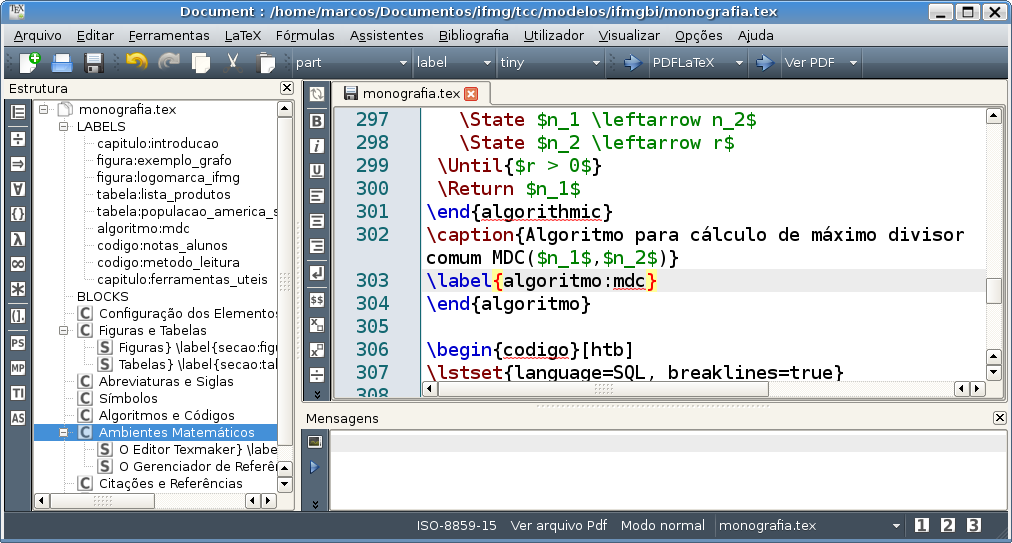
\includegraphics[width=\textwidth]{figuras/texmaker}
 \caption{Tela do Texmaker}
 \label{figura:texmaker}
\end{figure}

\begin{figure}[htb]
 \centering
 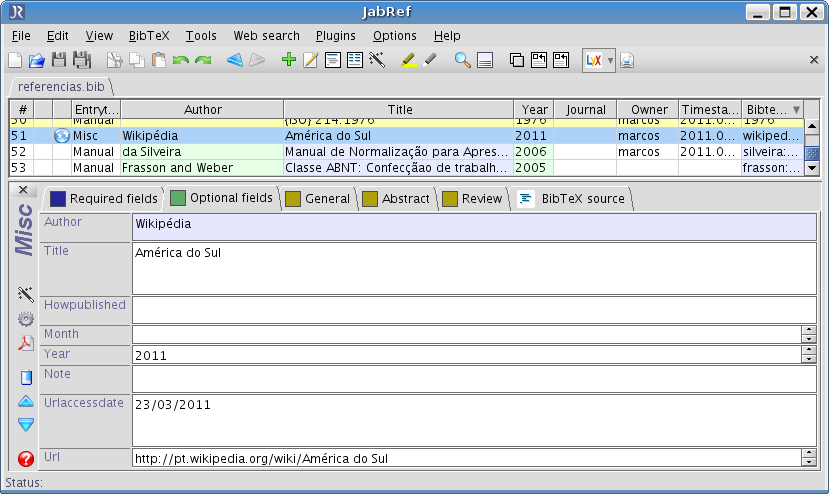
\includegraphics[width=\textwidth]{figuras/jabref}
 \caption{Tela do JabRef}
 \label{figura:jabref}
\end{figure}

O Texmaker pode ser obitido em \url{http://www.xm1math.net/texmaker} e o JabRef pode ser obtido em \url{http://www.jabref.org/}. É importante ressaltar que o Texmaker é apenas um editor, para compilar os documentos é necessário um ambiente Latex instalado. Os ambientes Latex mais populares são o Texlive (\url{http://www.tug.org/texlive}) e o MiKTex (\url{http://miktex.org}).
